\documentclass{standalone}
\usepackage{tikz}
\usetikzlibrary{patterns, positioning}

\begin{document}
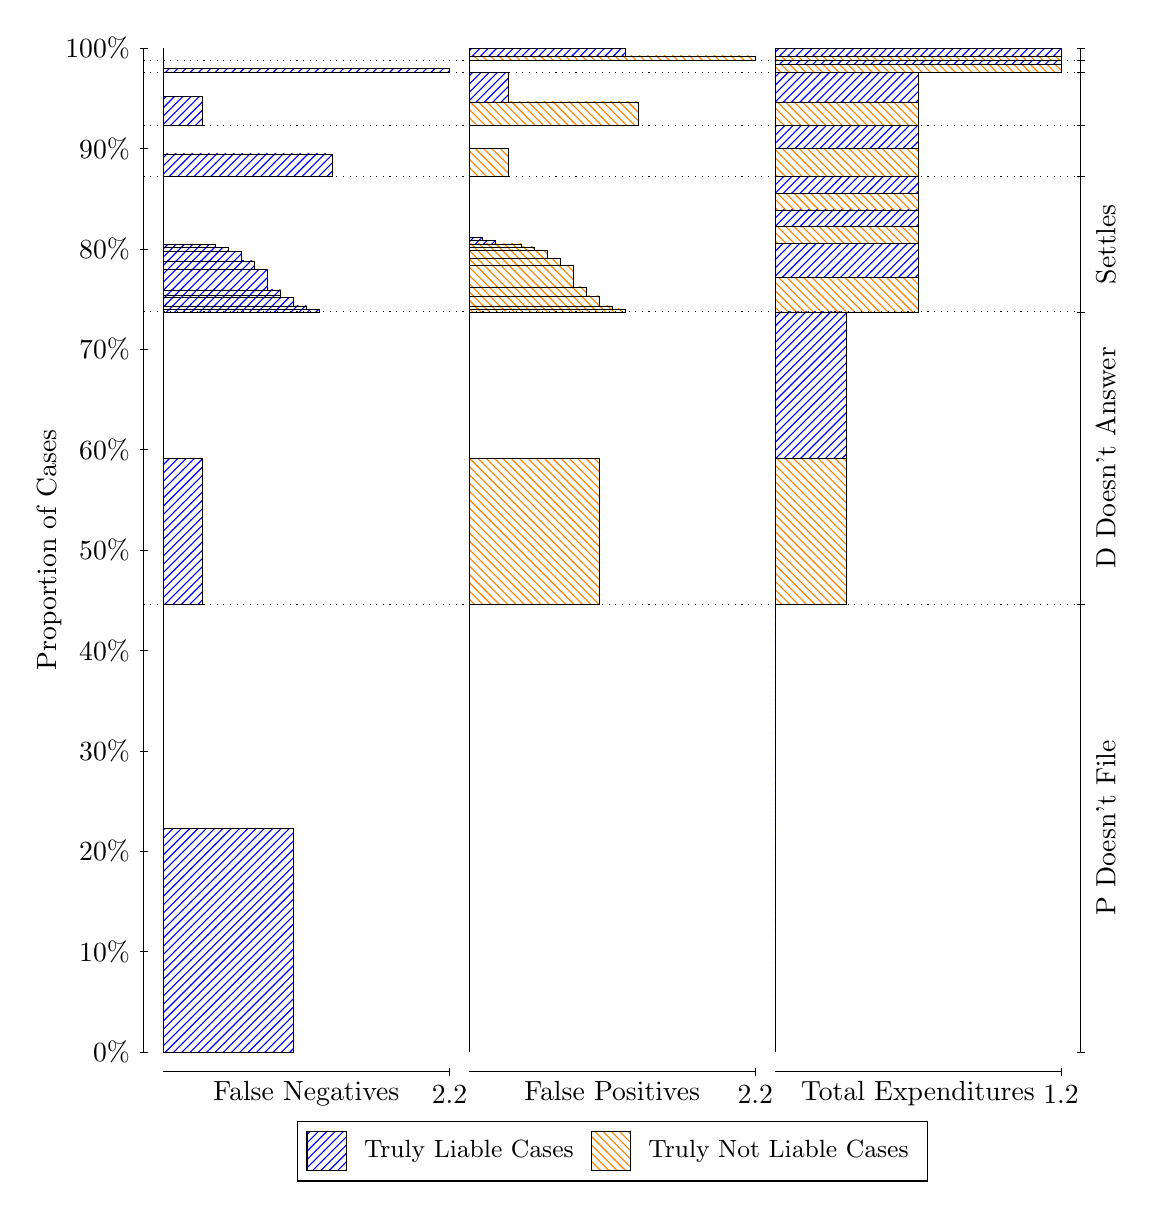
\begin{tikzpicture}
\draw[black, very thin] (1.5,1.75) -- (1.5,14.5);
\node[rotate=90, anchor=center] at (0.3, 8.125) {Proportion of Cases};
\draw[black, very thin] (1.45,1.75) -- (1.55,1.75);
\node[anchor=east] at (1.45, 1.75) {0\%};
\draw[black, very thin] (1.45,3.025) -- (1.55,3.025);
\node[anchor=east] at (1.45, 3.025) {10\%};
\draw[black, very thin] (1.45,4.3) -- (1.55,4.3);
\node[anchor=east] at (1.45, 4.3) {20\%};
\draw[black, very thin] (1.45,5.575) -- (1.55,5.575);
\node[anchor=east] at (1.45, 5.575) {30\%};
\draw[black, very thin] (1.45,6.85) -- (1.55,6.85);
\node[anchor=east] at (1.45, 6.85) {40\%};
\draw[black, very thin] (1.45,8.125) -- (1.55,8.125);
\node[anchor=east] at (1.45, 8.125) {50\%};
\draw[black, very thin] (1.45,9.4) -- (1.55,9.4);
\node[anchor=east] at (1.45, 9.4) {60\%};
\draw[black, very thin] (1.45,10.675) -- (1.55,10.675);
\node[anchor=east] at (1.45, 10.675) {70\%};
\draw[black, very thin] (1.45,11.95) -- (1.55,11.95);
\node[anchor=east] at (1.45, 11.95) {80\%};
\draw[black, very thin] (1.45,13.225) -- (1.55,13.225);
\node[anchor=east] at (1.45, 13.225) {90\%};
\draw[black, very thin] (1.45,14.5) -- (1.55,14.5);
\node[anchor=east] at (1.45, 14.5) {100\%};

\draw[black, very thin] (13.4,1.75) -- (13.4,14.5);
\draw[black, very thin] (13.35,1.75) -- (13.45,1.75);
\node[anchor=west] at (13.35, 1.75) {};
\draw[black, very thin] (13.35,7.4374) -- (13.45,7.4374);
\node[anchor=west] at (13.35, 7.4374) {};
\draw[black, very thin] (13.35,11.149) -- (13.45,11.149);
\node[anchor=west] at (13.35, 11.149) {};
\draw[black, very thin] (13.35,12.87) -- (13.45,12.87);
\node[anchor=west] at (13.35, 12.87) {};
\draw[black, very thin] (13.35,13.515) -- (13.45,13.515);
\node[anchor=west] at (13.35, 13.515) {};
\draw[black, very thin] (13.35,14.19) -- (13.45,14.19);
\node[anchor=west] at (13.35, 14.19) {};
\draw[black, very thin] (13.35,14.344) -- (13.45,14.344);
\node[anchor=west] at (13.35, 14.344) {};
\draw[black, very thin] (13.35,14.5) -- (13.45,14.5);
\node[anchor=west] at (13.35, 14.5) {};

\draw[black, very thin, pattern color=blue, pattern=north east lines] (1.75,1.75) rectangle (3.4015,4.5937);
\draw[black, very thin, pattern color=orange, pattern=north west lines] (1.75,4.5937) rectangle (1.75,7.4374);
\draw[black, very thin, pattern color=blue, pattern=north east lines] (1.75,7.4374) rectangle (2.2455,9.2931);
\draw[black, very thin, pattern color=orange, pattern=north west lines] (1.75,9.2931) rectangle (1.75,11.149);
\draw[black, very thin, pattern color=blue, pattern=north east lines] (1.75,11.149) rectangle (3.7318,11.185);
\draw[black, very thin, pattern color=blue, pattern=north east lines] (1.75,11.185) rectangle (3.5667,11.226);
\draw[black, very thin, pattern color=blue, pattern=north east lines] (1.75,11.226) rectangle (3.4015,11.335);
\draw[black, very thin, pattern color=blue, pattern=north east lines] (1.75,11.335) rectangle (3.2364,11.36);
\draw[black, very thin, pattern color=blue, pattern=north east lines] (1.75,11.36) rectangle (3.2364,11.429);
\draw[black, very thin, pattern color=blue, pattern=north east lines] (1.75,11.429) rectangle (3.0712,11.693);
\draw[black, very thin, pattern color=blue, pattern=north east lines] (1.75,11.693) rectangle (2.9061,11.796);
\draw[black, very thin, pattern color=blue, pattern=north east lines] (1.75,11.796) rectangle (2.7409,11.92);
\draw[black, very thin, pattern color=blue, pattern=north east lines] (1.75,11.92) rectangle (2.5758,11.965);
\draw[black, very thin, pattern color=blue, pattern=north east lines] (1.75,11.965) rectangle (2.4106,12.007);
\draw[black, very thin, pattern color=orange, pattern=north west lines] (1.75,12.007) rectangle (1.75,12.87);
\draw[black, very thin, pattern color=blue, pattern=north east lines] (1.75,12.87) rectangle (3.897,13.157);
\draw[black, very thin, pattern color=orange, pattern=north west lines] (1.75,13.157) rectangle (1.75,13.515);
\draw[black, very thin, pattern color=blue, pattern=north east lines] (1.75,13.515) rectangle (2.2455,13.889);
\draw[black, very thin, pattern color=orange, pattern=north west lines] (1.75,13.889) rectangle (1.75,14.19);
\draw[black, very thin, pattern color=blue, pattern=north east lines] (1.75,14.19) rectangle (5.3833,14.246);
\draw[black, very thin, pattern color=orange, pattern=north west lines] (1.75,14.246) rectangle (1.75,14.344);
\draw[black, very thin, pattern color=orange, pattern=north west lines] (1.75,14.344) rectangle (1.75,14.399);
\draw[black, very thin, pattern color=blue, pattern=north east lines] (1.75,14.399) rectangle (1.75,14.5);
\draw[black, very thin, pattern color=orange, pattern=north west lines] (5.6333,1.75) rectangle (5.6333,4.5937);
\draw[black, very thin, pattern color=blue, pattern=north east lines] (5.6333,4.5937) rectangle (5.6333,7.4374);
\draw[black, very thin, pattern color=orange, pattern=north west lines] (5.6333,7.4374) rectangle (7.2848,9.2931);
\draw[black, very thin, pattern color=blue, pattern=north east lines] (5.6333,9.2931) rectangle (5.6333,11.149);
\draw[black, very thin, pattern color=orange, pattern=north west lines] (5.6333,11.149) rectangle (7.6152,11.188);
\draw[black, very thin, pattern color=orange, pattern=north west lines] (5.6333,11.188) rectangle (7.45,11.225);
\draw[black, very thin, pattern color=orange, pattern=north west lines] (5.6333,11.225) rectangle (7.2848,11.352);
\draw[black, very thin, pattern color=orange, pattern=north west lines] (5.6333,11.352) rectangle (7.1197,11.466);
\draw[black, very thin, pattern color=orange, pattern=north west lines] (5.6333,11.466) rectangle (6.9545,11.739);
\draw[black, very thin, pattern color=orange, pattern=north west lines] (5.6333,11.739) rectangle (6.7894,11.825);
\draw[black, very thin, pattern color=orange, pattern=north west lines] (5.6333,11.825) rectangle (6.6242,11.93);
\draw[black, very thin, pattern color=orange, pattern=north west lines] (5.6333,11.93) rectangle (6.4591,11.974);
\draw[black, very thin, pattern color=orange, pattern=north west lines] (5.6333,11.974) rectangle (6.2939,12.012);
\draw[black, very thin, pattern color=blue, pattern=north east lines] (5.6333,12.012) rectangle (5.9636,12.054);
\draw[black, very thin, pattern color=blue, pattern=north east lines] (5.6333,12.054) rectangle (5.7985,12.099);
\draw[black, very thin, pattern color=blue, pattern=north east lines] (5.6333,12.099) rectangle (5.6333,12.87);
\draw[black, very thin, pattern color=orange, pattern=north west lines] (5.6333,12.87) rectangle (6.1288,13.229);
\draw[black, very thin, pattern color=blue, pattern=north east lines] (5.6333,13.229) rectangle (5.6333,13.515);
\draw[black, very thin, pattern color=orange, pattern=north west lines] (5.6333,13.515) rectangle (7.7803,13.816);
\draw[black, very thin, pattern color=blue, pattern=north east lines] (5.6333,13.816) rectangle (6.1288,14.19);
\draw[black, very thin, pattern color=orange, pattern=north west lines] (5.6333,14.19) rectangle (5.6333,14.288);
\draw[black, very thin, pattern color=blue, pattern=north east lines] (5.6333,14.288) rectangle (5.6333,14.344);
\draw[black, very thin, pattern color=orange, pattern=north west lines] (5.6333,14.344) rectangle (9.2667,14.399);
\draw[black, very thin, pattern color=blue, pattern=north east lines] (5.6333,14.399) rectangle (7.6152,14.5);
\draw[black, very thin, pattern color=orange, pattern=north west lines] (9.5167,1.75) rectangle (9.5167,4.5937);
\draw[black, very thin, pattern color=blue, pattern=north east lines] (9.5167,4.5937) rectangle (9.5167,7.4374);
\draw[black, very thin, pattern color=orange, pattern=north west lines] (9.5167,7.4374) rectangle (10.425,9.2931);
\draw[black, very thin, pattern color=blue, pattern=north east lines] (9.5167,9.2931) rectangle (10.425,11.149);
\draw[black, very thin, pattern color=orange, pattern=north west lines] (9.5167,11.149) rectangle (11.333,11.586);
\draw[black, very thin, pattern color=blue, pattern=north east lines] (9.5167,11.586) rectangle (11.333,12.02);
\draw[black, very thin, pattern color=orange, pattern=north west lines] (9.5167,12.02) rectangle (11.333,12.232);
\draw[black, very thin, pattern color=blue, pattern=north east lines] (9.5167,12.232) rectangle (11.333,12.443);
\draw[black, very thin, pattern color=orange, pattern=north west lines] (9.5167,12.443) rectangle (11.333,12.657);
\draw[black, very thin, pattern color=blue, pattern=north east lines] (9.5167,12.657) rectangle (11.333,12.87);
\draw[black, very thin, pattern color=orange, pattern=north west lines] (9.5167,12.87) rectangle (11.333,13.229);
\draw[black, very thin, pattern color=blue, pattern=north east lines] (9.5167,13.229) rectangle (11.333,13.515);
\draw[black, very thin, pattern color=orange, pattern=north west lines] (9.5167,13.515) rectangle (11.333,13.816);
\draw[black, very thin, pattern color=blue, pattern=north east lines] (9.5167,13.816) rectangle (11.333,14.19);
\draw[black, very thin, pattern color=orange, pattern=north west lines] (9.5167,14.19) rectangle (13.15,14.288);
\draw[black, very thin, pattern color=blue, pattern=north east lines] (9.5167,14.288) rectangle (13.15,14.344);
\draw[black, very thin, pattern color=orange, pattern=north west lines] (9.5167,14.344) rectangle (13.15,14.399);
\draw[black, very thin, pattern color=blue, pattern=north east lines] (9.5167,14.399) rectangle (13.15,14.5);
\draw[black, dotted] (1.5,7.4374) -- (13.4,7.4374);
\draw[black, dotted] (1.5,11.149) -- (13.4,11.149);
\draw[black, dotted] (1.5,12.87) -- (13.4,12.87);
\draw[black, dotted] (1.5,13.515) -- (13.4,13.515);
\draw[black, dotted] (1.5,14.19) -- (13.4,14.19);
\draw[black, dotted] (1.5,14.344) -- (13.4,14.344);
\draw[black, very thin] (1.75,1.5) -- (5.3833,1.5);
\node[anchor=north] at (3.5667, 1.5) {False Negatives};
\draw[black, very thin] (5.3833,1.45) -- (5.3833,1.55);
\node[anchor=north] at (5.3833, 1.45) {2.2};

\draw[black, very thin] (5.6333,1.5) -- (9.2667,1.5);
\node[anchor=north] at (7.45, 1.5) {False Positives};
\draw[black, very thin] (9.2667,1.45) -- (9.2667,1.55);
\node[anchor=north] at (9.2667, 1.45) {2.2};

\draw[black, very thin] (9.5167,1.5) -- (13.15,1.5);
\node[anchor=north] at (11.333, 1.5) {Total Expenditures};
\draw[black, very thin] (13.15,1.45) -- (13.15,1.55);
\node[anchor=north] at (13.15, 1.45) {1.2};

\node[black, centered, rotate=90] at (13.72, 4.5937) {P Doesn't File};
\node[black, centered, rotate=90] at (13.72, 9.2931) {D Doesn't Answer};
\node[black, centered, rotate=90] at (13.72, 12.009) {Settles};





\draw (7.449999999999999,1.5) node[draw=none] (baseCoordinate) {};
\begin{scope}[align=center]
        \matrix[scale=0.5, draw=black, below=0.5cm of baseCoordinate, nodes={draw}, column sep=0.1cm]{
            \node[rectangle, draw, minimum width=0.5cm, minimum height=0.5cm, pattern=north east lines, pattern color=blue] {}; &
            \node[draw=none, font=\small] (B) {Truly Liable Cases}; &
            \node[rectangle, draw, minimum width=0.5cm, minimum height=0.5cm, pattern=north west lines, pattern color=orange] {}; &
            \node[draw=none, font=\small] (B) {Truly Not Liable Cases}; \\
            };
\end{scope}

\end{tikzpicture}
\end{document}